\section{System Overview}
\label{sec:overview}

%An intuitive solution for the \emph{Text-to-Constraints} problem is to prompt an LLM with the entire document, schema, and sample records, asking it to extract constraints directly.
%\system\ also supports this mode, but in practice, it can be brittle when schemas are large or texts are long and loosely structured. Relevant text is usually scattered throughout the document, much of the content is unrelated to data or constraints, and so the prompt must simultaneously detect constraint-relevant text, align it with the schema, and generate constraints. Document-level processing also offers limited traceability, as identifying which part of the text justifies a given constraint is itself a separate task.

This section presents \system, our proposed framework for the Text-to-Constraints problem. 

Intuitively, one could address this problem with a single LLM prompt that includes the entire document, the dataset schema, and extraction instructions. Such a prompt, however, must jointly locate statements scattered across the text, align them with the schema, and build valid constraints, and it does not link each constraint to the text that justifies it; recovering this link requires an attribution step, such as summarizing related sentences and then mapping each summary.


We therefore decompose the problem into a pipeline that operates at the sentence level, processing each sentence individually. This design provides fine-grained traceability without an attribution step, since it links each constraint to the specific sentence that justifies it, and allows each component of the pipeline to be tuned independently.

\system\ takes as input a normative document, segmented into sentences, and a relational dataset and outputs sentence--constraint pairs. Figure~\ref{fig:pipeline} outlines the pipeline.

\begin{figure}[!ht]
\vspace{-10pt}
\centering
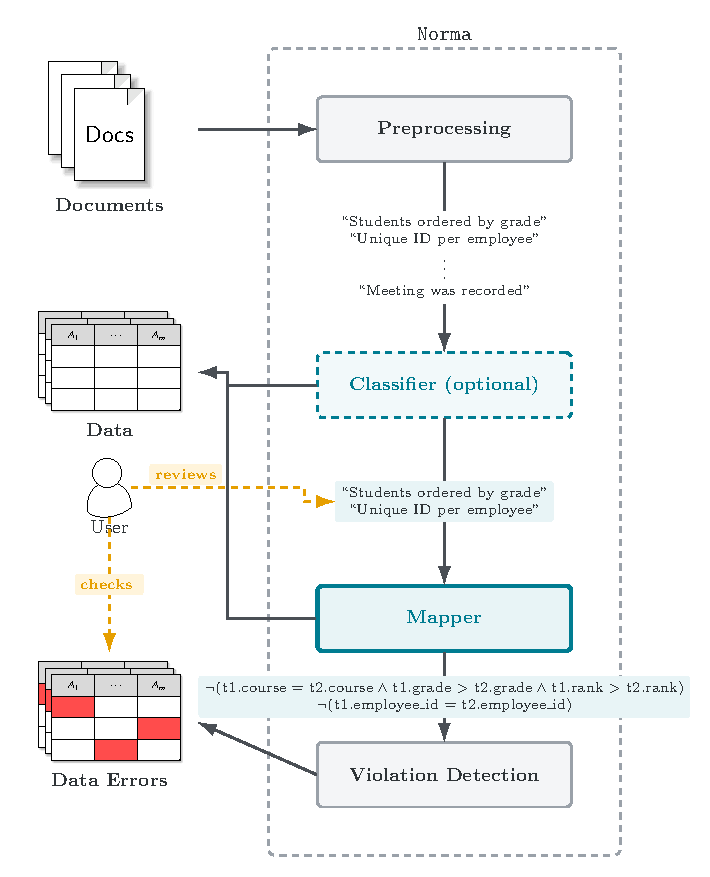
\includegraphics[width=\columnwidth]{diagramas/pipeline_norma.pdf}
%\caption{The \system\ pipeline.}
\vspace{-10pt}
\caption{Overview of the \system\ pipeline. Blue components represent the novel contributions presented in this paper.}
\label{fig:pipeline}
\vspace{-10pt}
\end{figure}

\smallskip\noindent\textbf{Preprocessing.}
An automated pipeline converts documents (e.g., PDF files) into normalized text: it extracts the text, removes hyphenation, normalizes whitespace, and segments sentences, followed by minimal manual cleanup. We treat this step as input preparation.


\smallskip\noindent\textbf{Constraint classifier.}
Given the sentences from preprocessing, a lightweight classifier can optionally identify those that likely express checkable constraints, filtering out content that is clearly unrelated to data quality constraints.  Since constraints missed at this stage cannot be recovered downstream, we prioritize recall at this stage. False positives can still be ruled out by the mapper (which we define next). The classifier only labels the given sentences and never generates text, so it preserves the link between each sentence and its constraint. When no classifier is used, all sentences are passed directly to the mapper. A user can optionally be involved at this stage, reviewing and correcting the set of classified sentences before proceeding to mapping. We describe the classifier details in Section~\ref{sec:classifier}.


\smallskip\noindent\textbf{Constraint mapper.}
The mapper is the central and most complex component of \system. It takes each sentence, optionally pre-filtered by the classifier, and produces a denial constraint grounded in the dataset schema.
It must interpret the sentence, align it with schema elements, and synthesize a constraint with correct violation semantics. Outputs that fail validation are rejected, and sentences that yield no valid constraint are excluded (Section~\ref{sec:mapper}).


\smallskip\noindent\textbf{Violation detection.}
Each constraint is validated by compiling it into a SQL violation query and executing it on the target relation (Section~\ref{sec:mapper:sql}), and it is linked back to the sentence that produced it. \system\ returns the violating tuples to the user for further inspection. DC violation detection is a well-studied problem, with specialized systems available for large-scale consistency checks~\cite{facet2021,liu2024rapidash,youri2024}. We compile DCs into SQL because the queries run on any engine that holds the data and also serve the data-based checks of the mapper; specialized engines can replace this step for larger workloads.


